\documentclass[xcolor={dvipsnames},handout]{beamer}

\usepackage{assets/pres-template_MOW}

%--------------------------------------------------------------------------
% Specific to this document ---------------------------------------
%--------------------------------------------------------------------------
% \setbeamercovered{transparent}

%%%%%%%%%%%%%%%%%%%%%%%%%%%%%%%%%%%
\setlength{\tabcolsep}{1.3pt}
\title{PLSC 48110/28110}
\subtitle{Lecture 1: Course introduction}
\date{}
\author{Molly Offer-Westort}
\institute{Department of Political Science, \\University of Chicago}


\usepackage{assets/Sweave}
\hypersetup{pdftitle={PLSC 48110/28110 - Lecture 1: Course introduction},pdfauthor={Molly Offer-Westort},pdfpagemode=UseNone}
\begin{document}

%-------------------------------------------------------------------------------%
\frame{\titlepage
\thispagestyle{empty}
}
%-------------------------------------------------------------------------------%
\begin{frame}{Overview}

This course:
\begin{itemize}
\item Objectives. 
\item Course structure. 
\item Final project. 
\end{itemize}
\vskip 0.5cm




Link to \href{../syllabus/syllabus.pdf}{syllabus}.

\end{frame}


%%%%%NOTE%%%%%
\note{
\scriptsize \singlespacing

\begin{itemize}
\item xxxx
\end{itemize}

}

%-------------------------------------------------------------------------------%
%%% [[TEMPLATE]] %%%
\begin{frame}[c]{}

How do we think about how experiments contribute to (social) scientific knowledge?

\end{frame}


%%%%%NOTE%%%%%
\note{
\scriptsize \singlespacing

\begin{itemize}
\item xxxx
\end{itemize}

}

%-------------------------------------------------------------------------------%
\begin{frame}{Reading papers}

 What to get out of reading a research paper:
\begin{itemize}
\item What is the main question of the paper?
\item What method do the authors use to address the question?
For empirical papers:
\begin{itemize}
\item Data (Where does it come from/how is it generated? What is the sample population? What is being measured?)
\item Research design/strategy
\item Statistical tools
\end{itemize}
{
\item What is the answer that the authors get to the main question?}
\end{itemize}

\end{frame}


%%%%%NOTE%%%%%
\note{
\scriptsize \singlespacing

\begin{itemize}
\item xxxx
\end{itemize}

}

%-------------------------------------------------------------------------------%
\begin{frame}{Proposing theories [KKV]}

\citep{king2021designing}

\begin{itemize}
\item Propose theories that are \textit{falsifiable}.
\item If you want to be able to test this theory, it should have \textit{observable implications}. (The more the better.) \
\item Clarity and precision in your theory is helpful. 
\end{itemize}

\end{frame}


%%%%%NOTE%%%%%
\note{
\scriptsize \singlespacing

\begin{itemize}
\item xxxx
\end{itemize}

}

%-------------------------------------------------------------------------------%
\begin{frame}{Reading papers}

What to get out of reading a research paper:
\begin{itemize}
\item What is the main question of the paper?
\item What method do the authors use to address the question?
{For empirical papers:}
\begin{itemize}
\item Data (Where does it come from/how is it generated? What is the sample population? What is being measured?)\
\item Research design/strategy
\item Statistical tools
\end{itemize}
\item What is the answer that the authors get to the main question?
\end{itemize}

\end{frame}


%%%%%NOTE%%%%%
\note{
\scriptsize \singlespacing

\begin{itemize}
\item xxxx
\end{itemize}

}

%-------------------------------------------------------------------------------%
\begin{frame}{How does this inform how we think about data?}

\begin{itemize}
\item Data is not something that is handed down to us in its complete and final form--we select and shape our data. 
\end{itemize}

\end{frame}


%%%%%NOTE%%%%%
\note{
\scriptsize \singlespacing

\begin{itemize}
\item xxxx
\end{itemize}

}

%-------------------------------------------------------------------------------%
\begin{frame}{Principles of data collection [KKV]}

\begin{enumerate}
\item Record and report data generation process.
\item Collect data on as many observable implications as possible. 
\item Maximize the validity of measurements. 
\item Ensure that data-collection methods are reliable.
\item Data and analyses should be as replicable as possible. 
\end{enumerate}

\end{frame}


%%%%%NOTE%%%%%
\note{
\scriptsize \singlespacing

\begin{itemize}
\item What does it mean to maximize validity of measurements?
\end{itemize}

}
%-------------------------------------------------------------------------------%
\begin{frame}{Observable implications}

\begin{itemize}
\item What are these?
\item How do observable implications relate to causal inference?
\end{itemize}

\end{frame}


%%%%%NOTE%%%%%
\note{
\scriptsize \singlespacing

\begin{itemize}
\item xxxx
\end{itemize}

}

%-------------------------------------------------------------------------------%
\begin{frame}{Inference}

\begin{itemize}
\item What is descriptive inference?
\item What is causal inference?
\end{itemize}

\end{frame}


%%%%%NOTE%%%%%
\note{
\scriptsize \singlespacing

\begin{itemize}
\item xxxx
\end{itemize}

}

%-------------------------------------------------------------------------------%
\begin{frame}{Elements of (descriptive/causal) inference [Holland]}
\citep{holland1986statistics}

\begin{itemize}
\item Define a population of interest. $U$
\item Determine a variable that is defined over this population, for which there is variation. $A$
\item Define response variable ``of interest.'' $Y$ 
\end{itemize}

We can consider how $A$ and $Y$ vary together. Without further assumptions, this is just correlation. 

\end{frame}


%%%%%NOTE%%%%%
\note{
\scriptsize \singlespacing

\begin{itemize}
\item xxxx
\end{itemize}

}

%-------------------------------------------------------------------------------%
\begin{frame}

\begin{center}
What does it mean for something to cause something else?
\end{center}

\end{frame}


%%%%%NOTE%%%%%
\note{
\scriptsize \singlespacing

\begin{itemize}
\item xxxx
\end{itemize}

}

%-------------------------------------------------------------------------------%
\begin{frame}{What does it mean for something to cause something else? [Rubin]}
\citep{rubin1974estimating,rubin1977assignment, rubin1978bayesian, rubin1980discussion, holland1980causal}

\begin{itemize}
\item Possibility for multiple values of treatment--\textit{for each individual}. Treatment \textit{could have been different}. $S(u) = t$ OR $S(u) = c$
\item Some temporal element: outcome variable is realized after ``exposure'' to treatment variable. $S(u)\rightarrow Y(u)$
\item Conceptual possibility for multiple different versions of response variable--\textit{for each individual}. $Y_t(u)$ may not equal $Y_c(u)$
\end{itemize}
Consider the individual \textit{causal effect}
\[
Y_t(u)-Y_c(u).
\]
\end{frame}


%%%%%NOTE%%%%%
\note{
\scriptsize \singlespacing

\begin{itemize}
\item xxxx
\end{itemize}

}

%-------------------------------------------------------------------------------%
\begin{frame}{No causation without manipulation [Holland]}

\begin{itemize}
\item Causes are only things that could (hypothetically) be treatments in experiments. 
\item NOT attributes--e.g., race and biological sex can't plausibly be manipulated, because there is no meaningful \textit{counterfactual}. 
\begin{itemize}
\item What we can manipulate: others' \textit{perception} of race/sex (e.g., audit experiments)%\citep{bertrand2004emily} 

\item To the extent that sex/gender are social constructs, can we consider counterfactual socialization?
\end{itemize}
\end{itemize}

\end{frame}


%%%%%NOTE%%%%%
\note{
\scriptsize \singlespacing

\begin{itemize}
\item xxxx
\end{itemize}

}

%-------------------------------------------------------------------------------%
\begin{frame}{Fundamental problem of causal inference}

\begin{itemize}
\item We only see the response variable under one version of treatment.
\item Why does this matter?
\end{itemize}

\end{frame}


%%%%%NOTE%%%%%
\note{
\scriptsize \singlespacing

\begin{itemize}
\item xxxx
\end{itemize}

}

%-------------------------------------------------------------------------------%
\begin{frame}{Resolution (?) of the fundamental problem of causal inference}

\begin{itemize}
\item Causal inference is not impossible. 
\item But making causal inferences without making assumptions IS impossible. 
\item So we need to depend on some assumptions. 
\item The crux: how plausible are these assumptions?
\end{itemize}

\end{frame}


%%%%%NOTE%%%%%
\note{
\scriptsize \singlespacing

\begin{itemize}
\item xxxx
\end{itemize}

}

%-------------------------------------------------------------------------------%
\begin{frame}{Some special cases of causal inference}

\begin{itemize}
\item Temporal stability 
\item Causal transience 
\item Unit homogeneity 
\item Constant causal effect 
\item Independence
\end{itemize}

\end{frame}


%%%%%NOTE%%%%%
\note{
\scriptsize \singlespacing

\begin{itemize}
\item xxxx
\end{itemize}

}

%-------------------------------------------------------------------------------%
\begin{frame}{Temporal stability and causal transience}

\begin{itemize}
\item The value of response will not change based on \textit{when} you apply treatment to an observation. 
\item The value of response will not change if you had at some point previously applied a different treatment to an observation. 
\end{itemize}

\end{frame}


%%%%%NOTE%%%%%
\note{
\scriptsize \singlespacing

\begin{itemize}
\item xxxx
\end{itemize}

}

%-------------------------------------------------------------------------------%
\begin{frame}{Unit homogeneity}

\begin{itemize}
\item The value of response under a given treatment is the same for two observations; and the value of response for a different treatment is also the same. 
\item You can observe response on the comparable units under one of each version of treatment. 
\end{itemize}

\end{frame}


%%%%%NOTE%%%%%
\note{
\scriptsize \singlespacing

\begin{itemize}
\item xxxx
\end{itemize}

}

%-------------------------------------------------------------------------------%
\begin{frame}{Constant causal effect}

\begin{itemize}
\item The difference between the value of the response variable under one version of treatment as compared to another version of treatment is the same for \textit{every} observation. 
\item How does this relate to the unit homogeneity assumption? 
\item Does this allow us to back out the value of the causal effect, without other assumptions?
\end{itemize}

\end{frame}


%%%%%NOTE%%%%%
\note{
\scriptsize \singlespacing

\begin{itemize}
\item xxxx
\end{itemize}

}

%-------------------------------------------------------------------------------%
\begin{frame}{Independence}

\begin{itemize}
\item There are a ``large'' number of observations. 
\item On average, the units that are assigned one version of treatment look like the units that receive another version of treatment. %
% \item (What does $\textrm{E}[Y_s |S = t]$ mean?)
\end{itemize}

\end{frame}


%%%%%NOTE%%%%%
\note{
\scriptsize \singlespacing

\begin{itemize}
\item xxxx
\end{itemize}

}

%-------------------------------------------------------------------------------%
% \begin{frame}{Independence}
% 
% \begin{itemize}
% \item Units that receive treatment look, on average, like units that do not. 
% \item In experiments, we assign treatment \textit{randomly}, so we know that there is no inherent difference between subjects that \textit{could have} received treatment and \textit{could have} received control--all subjects \textit{could have} received all versions of treatment, hypothetically. (The subjunctive mood of research design \dots)
% \item Why is this so special? 
% \item What this give us: $\E[Y_i | W_i = 0] = \E[Y_i(1)]$ 
% \item We can back out an estimate of the average treatment effect:
% $$
% \tau = \E[Y_i(1)-Y_i(0)]
% $$
% \end{itemize}
% 
% \end{frame}
% 
% 
% %%%%%NOTE%%%%%
% \note{
% \scriptsize \singlespacing
% 
% \begin{itemize}
% \item xxxx
% \end{itemize}
% 
% }

%-------------------------------------------------------------------------------%

\begin{frame}{The special role of experiments}

\begin{itemize}
\item In experiments, treatment is randomly assigned by the researcher. 
\item So we know independence holds by design.  
\item We can compare groups and get the \textit{average} causal effect. 
\item (When can we also get the \textit{individual} causal effect?) 
\end{itemize}

\end{frame}


%%%%%NOTE%%%%%
\note{
\scriptsize \singlespacing

\begin{itemize}
\item xxxx
\end{itemize}

}


%-------------------------------------------------------------------------------%
\begin{frame}{An aside on Nobels}

\begin{figure}
\centering
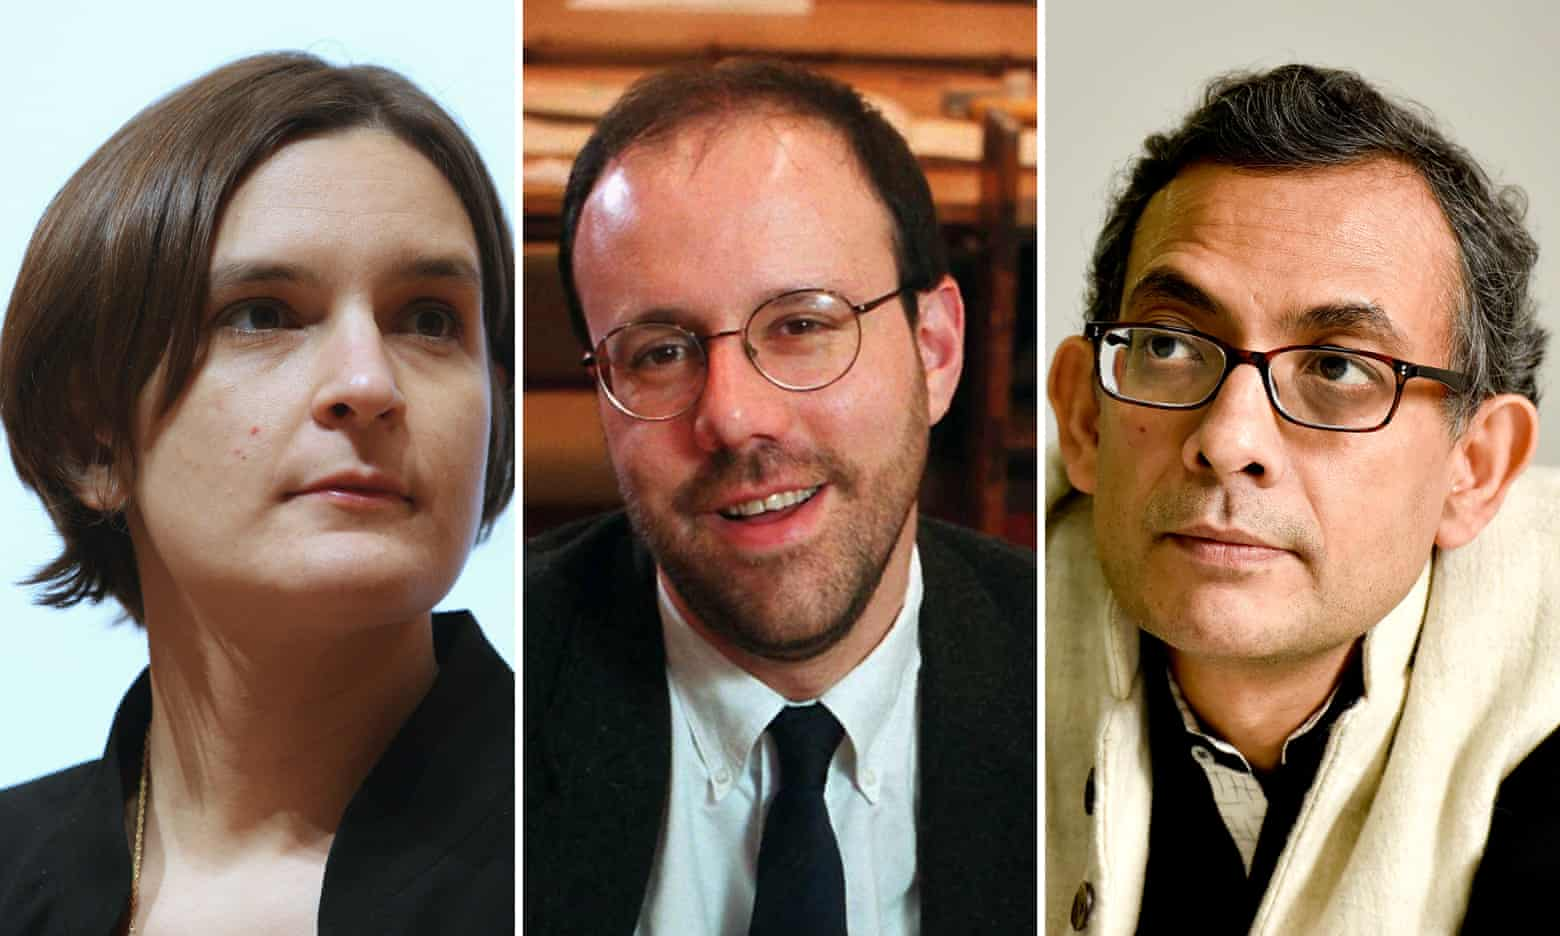
\includegraphics{assets/nobels19.jpeg}
\caption{Esther Duflo, Michael Kremer, and Abhijit Banerjee}
\end{figure}

\end{frame}


%%%%%NOTE%%%%%
\note{
\scriptsize \singlespacing

\begin{itemize}
\item xxxx
\end{itemize}

}

%-------------------------------------------------------------------------------%
\begin{frame}{An aside on Nobels}

2019 economics nobel awarded for: ``their experimental approach to alleviating global poverty.'' \ Why is this a big deal? 
\begin{itemize}
\item One way to understand human behavior: posit a theory. E.g., propose a utility function.  
\item[$\rightarrow$] Deduce implications of theory. 
\item[$\rightarrow$] (maybe) Test implications against data.  
\item[$\rightarrow$] Update and revise theory. 
\end{itemize}

\end{frame}


%%%%%NOTE%%%%%
\note{
\scriptsize \singlespacing

\begin{itemize}
\item xxxx
\end{itemize}

}

%-------------------------------------------------------------------------------%
\begin{frame}{Experiments}

How do we know if policies are working? 
\begin{itemize}
\item Duflo, Banerjee, Kremer motivated by work of development agencies. 
\item Interventions are large scale, complicated, and hard to deduce how ``effective'' they should be based on theory alone. 
\item A solution: build rigorous evidence for policy efficacy. 
\item One way to build evidence: experiments. 
\end{itemize}

\end{frame}


%%%%%NOTE%%%%%
\note{
\scriptsize \singlespacing

\begin{itemize}
\item xxxx
\end{itemize}

}

%-------------------------------------------------------------------------------%
\backupbegin
%-------------------------------------------------------------------------------%

\begin{frame}[allowframebreaks]{References}
    \bibliographystyle{apalike}
    \bibliography{assets/bib}
\end{frame}
%-------------------------------------------------------------------------------%
\backupend
\end{document}
